\documentclass[journal, onecolumn, 12pt]{IEEEtran}
\IEEEoverridecommandlockouts

\usepackage{amsmath, amssymb}
\usepackage{graphicx}
\usepackage{booktabs}
\usepackage{float}
\usepackage{cite}
\usepackage{caption}
\usepackage{textcomp}
\usepackage{url}

\begin{document}

\title{Physics-Constrained Machine Learning for Predictive Modeling of a Coupled Forward Osmosis-Reverse Osmosis Textile Wastewater Process}

\author{
\IEEEauthorblockN{First Author, Second Author, and Third Author}
\IEEEauthorblockA{
\textit{Department of Chemical Engineering}\\
\textit{Advanced Membrane Technologies Laboratory}\\
Email: first.author@email.com, second.author@email.com, third.author@email.com
}
}

\maketitle

\begin{abstract}
Coupled forward osmosis-reverse osmosis (FO-RO) treatment has recently been demonstrated as a promising route for textile wastewater concentration, draw-solution regeneration, and clean-water recovery. The base experimental study used an Aquaporin HFFO14 forward-osmosis membrane and a DuPont SW30-2540 reverse-osmosis membrane to concentrate real end-of-pipe textile wastewater while continuously regenerating a 0.7 M NaCl draw solution. Although the experimental work established stable operation and high organic rejection, the resulting process data also provide a useful test case for predictive modeling under conditions that are difficult for generic machine-learning workflows: time-correlated flux data, very small calibration sets, and strict physical constraints on membrane behavior. In this project, the reported FO-RO data were reanalyzed using a set of model choices matched to the structure of each dataset. For the long-term FO flux record, temporal feature engineering improved the chronological holdout $R^2$ from $-0.055$ to $0.566$. For the sparse short-term FO flux dataset ($n=11$), Gaussian Process Regression improved leave-one-out cross-validation (LOOCV) performance from $R^2=0.425$ and RMSE $=1.133$ to $R^2=0.587$ and RMSE $=0.960$ while adding uncertainty bounds. For RO conductivity rejection, a two-parameter solution-diffusion model replaced an unconstrained polynomial and preserved physically meaningful extrapolation outside the 30--50 bar calibration range. Finally, per-stream solute models showed that no single regression form is optimal for TOC, TDS, and conductivity across feed and draw streams. These results show that membrane-process machine learning is most reliable when validation strategy, sample size, and transport physics are treated as part of the model design.
\end{abstract}

\begin{IEEEkeywords}
Forward osmosis, reverse osmosis, textile wastewater, machine learning, Gaussian Process Regression, solution-diffusion model, time-series validation.
\end{IEEEkeywords}

\section{Introduction}
Textile wastewater is typically characterized by high salinity, persistent organic compounds, color, conductivity, and variable organic loading \cite{b1,b2,b3}. Conventional dye-removal and wastewater-treatment approaches can reduce specific pollutant classes, but textile effluents remain challenging because of their mixed dye, salt, organic, and heavy-metal content \cite{b4,b5}. Membrane processes are attractive for this application because they can support water reuse and contaminant concentration without relying only on chemical destruction or disposal \cite{b1,b6,b7}. A recent experimental study demonstrated a coupled FO-RO system in which real end-of-pipe textile wastewater was concentrated by forward osmosis while the saline draw solution was continuously regenerated by reverse osmosis \cite{b1}. The process used a HFFO14 FO membrane with 13.8 m$^2$ active area and a SW30-2540 RO membrane with 2.8 m$^2$ active area. The draw solution was 0.7 M NaCl, and the wastewater was first concentrated to 90\% water recovery before the previously concentrated stream was treated again in a longer-term run \cite{b1}.

The treatment of textile wastewater is especially difficult because the wastewater composition is not fixed. Equalization-tank effluent can contain diluted residues from dyeing, washing, finishing, rinsing, and auxiliary chemical use, so the same treatment unit may experience changes in conductivity, organic loading, pH, and suspended or colloidal matter over time. This variability limits the value of single-point performance indicators. A membrane system that appears stable under one operating condition may behave differently when osmotic pressure, fouling tendency, or solute accumulation changes. For this reason, predictive models are useful only if they represent the physical and temporal structure of the process rather than merely fitting averaged experimental values.

Forward osmosis is attractive for concentrating wastewater because the driving force is an osmotic pressure gradient rather than direct hydraulic pressure. This can reduce compaction-related stress on the FO membrane and can make the process suitable for challenging feeds. However, FO performance depends strongly on draw-solution concentration, reverse salt flux, concentration polarization, membrane formulation, and fouling near the membrane surface \cite{b7,b10,b11,b12,b13,b14}. As water permeates from the feed to the draw side, the draw solution becomes diluted unless it is regenerated. Reverse osmosis can restore the draw-solution concentration and recover clean permeate, but it introduces its own pressure-dependent transport behavior, rejection limits, and energy considerations \cite{b6,b7}. A coupled FO-RO process therefore has two interacting membrane units rather than one isolated separation step.

In such a hybrid process, the main engineering variables are linked. FO permeate flux affects how quickly the wastewater becomes concentrated, while RO rejection and permeate flow determine whether the draw solution remains strong enough to sustain the osmotic driving force. Changes in conductivity, temperature, transmembrane pressure, feed concentration, and cleaning events can all alter the observed flux trajectory. These interactions make the dataset valuable for machine-learning analysis, but they also make it unsafe to treat all observations as independent, identically distributed samples. Time-ordered membrane data often contain autocorrelation, process events, and delayed effects that can make random cross-validation overly optimistic.

The base paper established the engineering feasibility of the process: FO operation maintained useful permeate flux, the RO unit regenerated the draw solution, and COD/TOC rejection remained above 99\% \cite{b1}. This is consistent with the broader development of FO membranes and FO-RO hybrid systems, where draw-solution selection, concentration polarization, reverse salt transport, and fouling behavior strongly affect process feasibility \cite{b7,b10,b11,b14}. However, the predictive modeling problem remains nontrivial. The available datasets are heterogeneous: the long-term FO record contains hundreds of autocorrelated observations, the short-term FO run has only 11 measured flux points, the RO rejection calibration contains only three pressure levels, and the solute-tracking dataset contains small per-stream series across recovery levels. Prior membrane-machine-learning studies show that data-driven models can predict membrane-system behavior, but their reliability depends strongly on data quality, validation design, and the structure of the process being modeled \cite{b15}. Applying one general-purpose machine-learning algorithm to all four problems would therefore be statistically fragile and, in some cases, physically misleading.

Another challenge is sample size. The long-term FO flux record contains enough observations to support feature engineering and chronological validation, but the short-term FO dataset contains only 11 points and the RO calibration contains only three pressure levels. Under these conditions, flexible models can easily describe the measured points while failing between or beyond them. This is particularly important for RO rejection, where a polynomial may interpolate the calibration range but predict physically unreasonable behavior below the osmotic-pressure threshold or outside the measured pressure window. Likewise, solute tracking across feed-in, feed-out, and draw-out streams cannot be forced into one universal regression form because each stream follows a different physical role in the coupled system.

This project reinterprets the base experimental data as a modeling case study. The objective is not to replace the membrane interpretation of the original work, but to show how process-aware machine-learning choices can improve prediction and prevent common errors such as temporal leakage, overfitting on sparse data, and unphysical extrapolation. This emphasis is consistent with recent membrane-system ML discussions, where data quality, interpretability, transferability, and process context remain central barriers to reliable deployment \cite{b15}. Accordingly, the present study uses different models for different parts of the FO-RO system: time-series-aware Random Forest modeling for long-term FO flux, Gaussian Process Regression for sparse flux and solute datasets, and a solution-diffusion physical model for RO rejection. The central contribution is therefore methodological: it demonstrates how validation strategy, sample size, and membrane-transport physics can be integrated into a coherent predictive workflow for hybrid FO-RO wastewater treatment.

\section{Data and Modeling Approach}
\subsection{Source Data}
The analysis used the experimental data extracted from the base FO-RO study \cite{b1}. The principal data products were: short-term FO flux during concentration of real textile wastewater, long-term FO flux during treatment of previously concentrated wastewater, RO conductivity rejection at 30, 40, and 50 bar, and sample-analysis data for TOC, TDS, and conductivity across feed-in, feed-out, and draw-out streams. These water-quality indicators are commonly used to describe organic loading, salinity, and treatment performance in industrial wastewater analysis \cite{b8,b9}.

\begin{figure}[H]
\centering
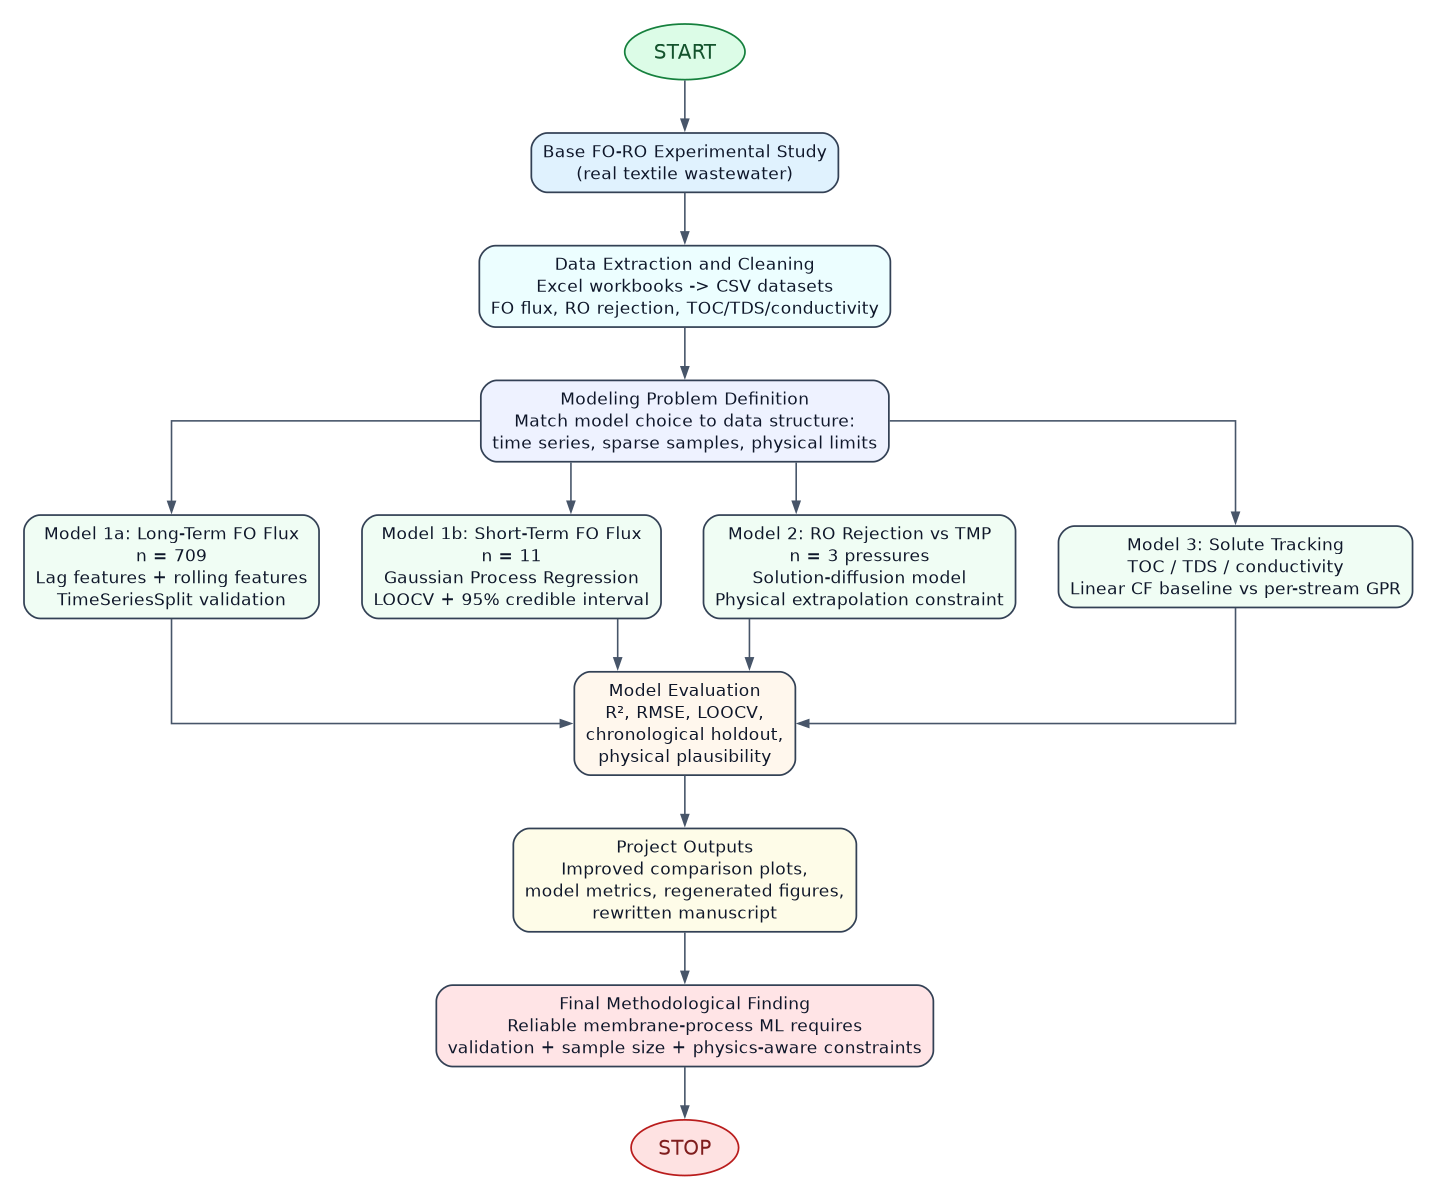
\includegraphics[width=0.95\linewidth]{plots/methodology_flow_diagram.png}
\caption{Methodology flow diagram for the physics-constrained machine-learning analysis of the coupled FO-RO textile wastewater treatment system.}
\label{fig:methodology_flow}
\end{figure}

\subsection{Model 1a: Long-Term FO Flux}
The long-term FO flux dataset contained 709 usable observations with time, conductivity, temperature, TMP, and flux-derived variables. A baseline Random Forest was first evaluated using the same strict chronological split used in the project notebooks: the first 75\% of the time series formed the training segment and the final 25\% formed the holdout segment. Additional engineered features were then added, including lagged flux values at 1, 3, and 5 steps, rolling conductivity and temperature summaries, rate-of-change terms, and a draw/feed conductivity ratio. Because prior FO modeling studies highlight the importance of process variables for flux prediction, these features were designed to retain both operating-condition and time-history information \cite{b1}. Because the data are time ordered, \texttt{TimeSeriesSplit} was used for cross-validation instead of random folds.

\subsection{Model 1b: Short-Term FO Flux}
The short-term FO dataset contained only 11 measured flux points. In this regime, tree-based ensembles are prone to step-function behavior between sparse observations. A Gaussian Process Regressor (GPR) was therefore used with a radial basis function component and a white-noise term, following the broader membrane-ML motivation of quantifying process behavior under limited measurements \cite{b1}. Model quality was evaluated by leave-one-out cross-validation, and the final plotted fit reports a 95\% credible interval.

\subsection{Model 2: RO Conductivity Rejection}
Only three calibration pressures were available for RO conductivity rejection: 30, 40, and 50 bar. A degree-2 polynomial can fit this range closely, but it has no transport constraint and can behave incorrectly outside the measured interval. The improved model therefore used a two-parameter solution-diffusion form, reflecting the need for physics-aware constraints in small-data process modeling \cite{b1} and the established pressure-driven transport interpretation of reverse osmosis \cite{b1,b6}:
\begin{equation}
R = 1 - \frac{B}{A(\Delta P-\Delta \pi)+B},
\end{equation}
where $A$ is a water-permeability parameter, $B$ is a salt-passage parameter, and $\Delta \pi$ was fixed at approximately 24.9 bar for the 0.5 M NaCl feed. The net driving pressure was bounded so that below the osmotic-pressure limit the model does not predict physically meaningful positive water flux.

\subsection{Model 3: TOC, TDS, and Conductivity Tracking}
For solute tracking, the baseline model used the concentration factor
\begin{equation}
CF=\frac{1}{1-\mathrm{recovery}/100}
\end{equation}
as the independent variable in linear regression. This is physically sensible for feed-side concentration, but it is not necessarily appropriate for the draw-out stream because the draw solution is continuously regenerated by RO and should not follow the same concentration factor as the feed. The improved workflow compared this baseline against per-stream GPR models fitted directly against water recovery percentage.

\section{Results and Discussion}
Table~\ref{tab:original_modified_overview} summarizes the main differences between the original experimental interpretation and the modified modeling workflow developed in this project. The original paper primarily reported measured membrane-process behavior, while the present work used the same extracted datasets to test predictive models, validation strategies, and physically constrained extrapolation.

\begin{table}[H]
\centering
\caption{Comparison between the original research paper results and the modified project results.}
\label{tab:original_modified_overview}
\begin{tabular}{p{0.19\linewidth}p{0.34\linewidth}p{0.34\linewidth}}
\toprule
Aspect & Original research paper & Modified project result \\
\midrule
Long-term FO flux & Reported stable FO permeate flux of approximately 3.9--4.1 L/h$\cdot$m$^2$ during treatment of previously concentrated wastewater. & Re-modeled the long-term flux time series using chronological validation. Temporal feature engineering improved holdout $R^2$ from $-0.055$ to $0.566$. \\
Short-term FO flux & Reported the measured decline in FO permeate flux as recovery increased toward 90\%. & Compared sparse-data models. GPR improved LOOCV performance from $R^2=0.425$, RMSE $=1.133$ to $R^2=0.587$, RMSE $=0.960$, with uncertainty bounds. \\
RO rejection & Reported high NaCl/conductivity rejection at 30, 40, and 50 bar, with approximately 99.2\% rejection at 50 bar. & Replaced unconstrained polynomial extrapolation with a solution-diffusion model. At 50 bar, the physical model predicted 99.40\%; at 70 bar, it remained bounded at 99.67\%; below osmotic pressure, it returned near-zero flux behavior. \\
TOC/TDS/conductivity & Reported feed, draw, and permeate water-quality behavior across recovery levels, with COD/TOC rejection above 99\%. & Compared linear concentration-factor regression with per-stream GPR. Results showed that feed streams and draw-out streams require different modeling assumptions. \\
Main contribution & Demonstrated experimental feasibility of simultaneous FO-RO treatment for real textile wastewater. & Converted the experimental dataset into a predictive, validation-aware, physics-constrained modeling workflow. \\
\bottomrule
\end{tabular}
\end{table}

\subsection{Long-Term FO Flux Prediction}
The base paper reported that, during longer-term treatment of previously concentrated wastewater, FO permeate flux remained stable at approximately 3.9--4.1 L/h$\cdot$m$^2$. The project data confirmed this broad trend but showed that a predictive model must also account for local time-series behavior and the final cleaning-event region. The baseline Random Forest achieved a chronological holdout $R^2$ of $-0.055$, indicating that it did not generalize well to the final holdout segment. Adding temporal features improved the holdout $R^2$ to $0.566$.

\begin{figure}[H]
\centering
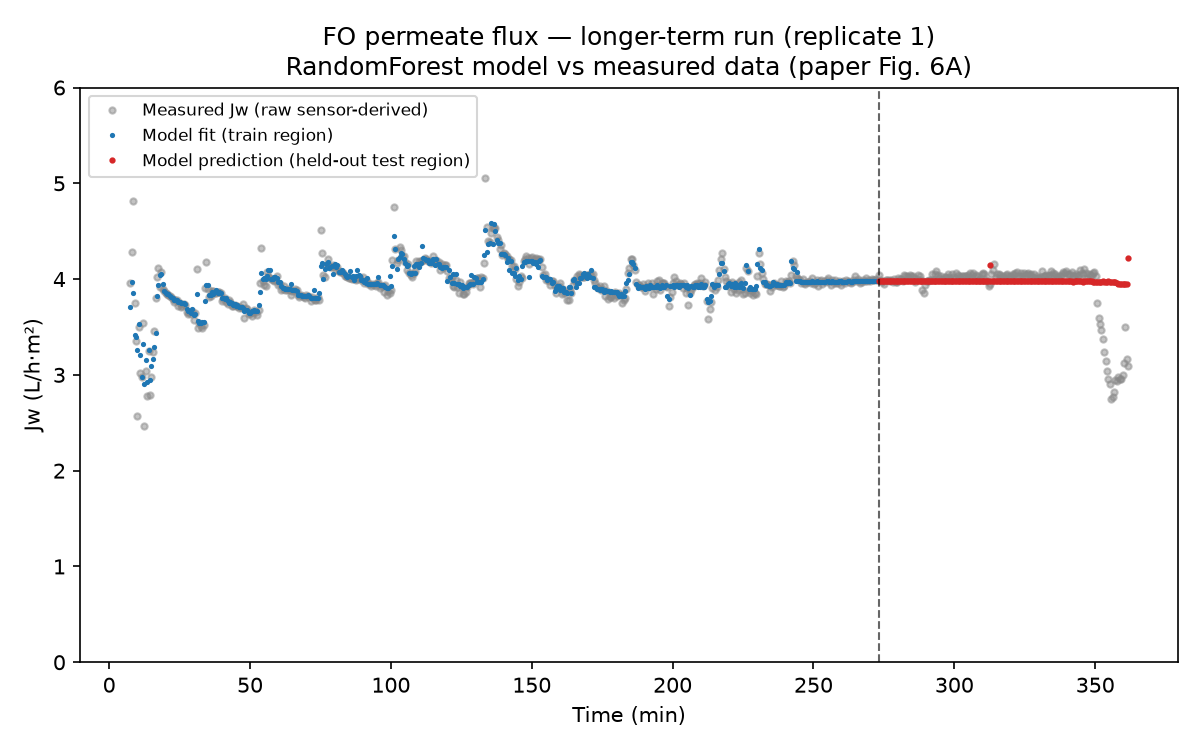
\includegraphics[width=0.92\linewidth]{plots/model1a_fo_flux_longterm.png}
\caption{Long-term FO permeate flux during treatment of previously concentrated textile wastewater, corresponding to the base paper's Fig. 6A.}
\label{fig:longterm_base}
\end{figure}

\begin{figure}[H]
\centering
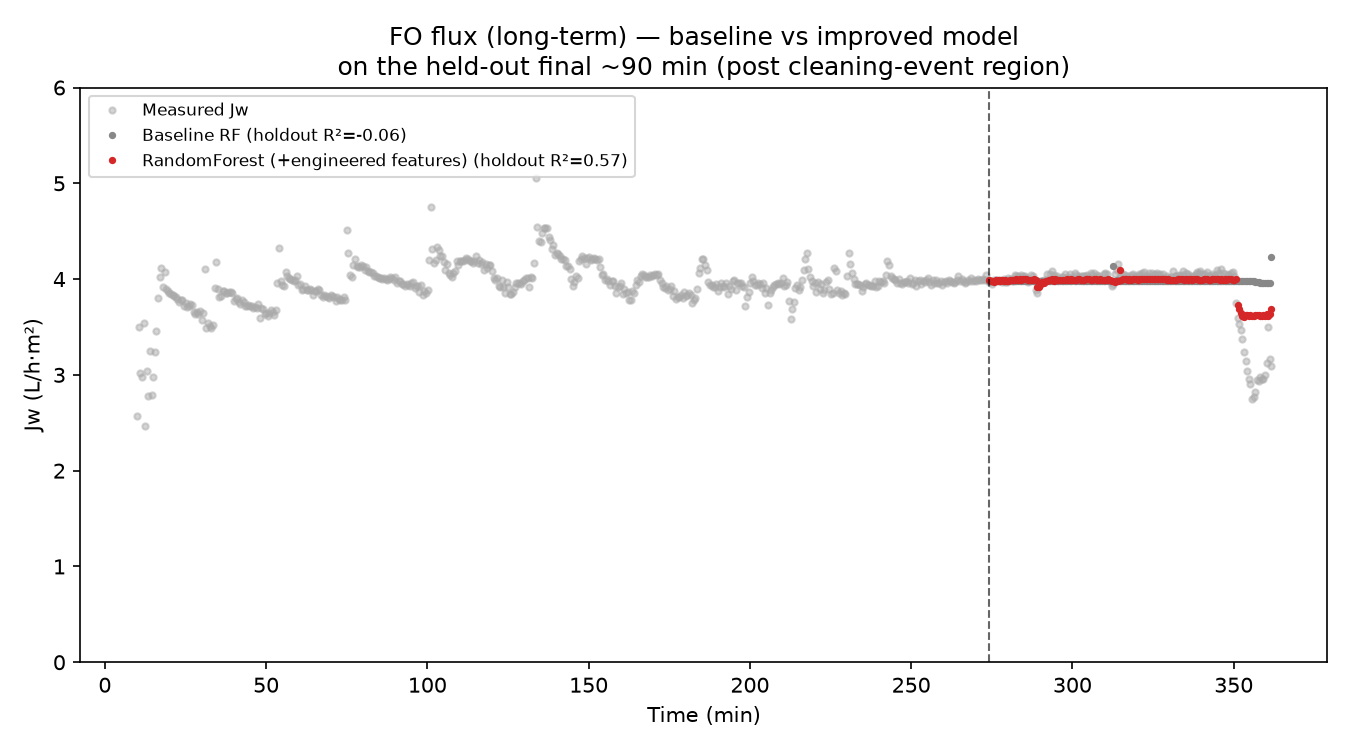
\includegraphics[width=0.92\linewidth]{plots/model1a_improved_comparison.png}
\caption{Chronological holdout prediction for long-term FO flux. Temporal feature engineering improved the Random Forest holdout $R^2$ from $-0.055$ to $0.566$.}
\label{fig:longterm_improved}
\end{figure}

\begin{table}[H]
\centering
\caption{Long-term FO flux model comparison.}
\label{tab:longterm_models}
\begin{tabular}{lcc}
\toprule
Model & Holdout $R^2$ & TimeSeriesSplit mean $R^2$ \\
\midrule
Random Forest, baseline features & $-0.055$ & $-3.575$ \\
Random Forest, engineered features & $0.566$ & $-0.054$ \\
HistGradientBoosting, tuned & $0.386$ & $-0.057$ \\
XGBoost, tuned & $0.323$ & $-0.399$ \\
\bottomrule
\end{tabular}
\end{table}

The key improvement was not simply changing to a more complex estimator. In fact, the best holdout result came from the Random Forest with better temporal features. The negative TimeSeriesSplit scores also show that this process remains difficult to forecast into some future intervals, especially where operating events alter the flux trajectory.

\subsection{Short-Term FO Flux Under Sparse Sampling}
The short-term FO run exhibits a clear flux decline as recovery increases and the cartridge filter approaches saturation. The baseline Gradient Boosting model produced LOOCV $R^2=0.425$ with RMSE $=1.133$. The GPR model improved the LOOCV score to $R^2=0.587$ and reduced RMSE to $0.960$. More importantly, the GPR expresses uncertainty directly, which is essential when only 11 points are available.

\begin{figure}[H]
\centering
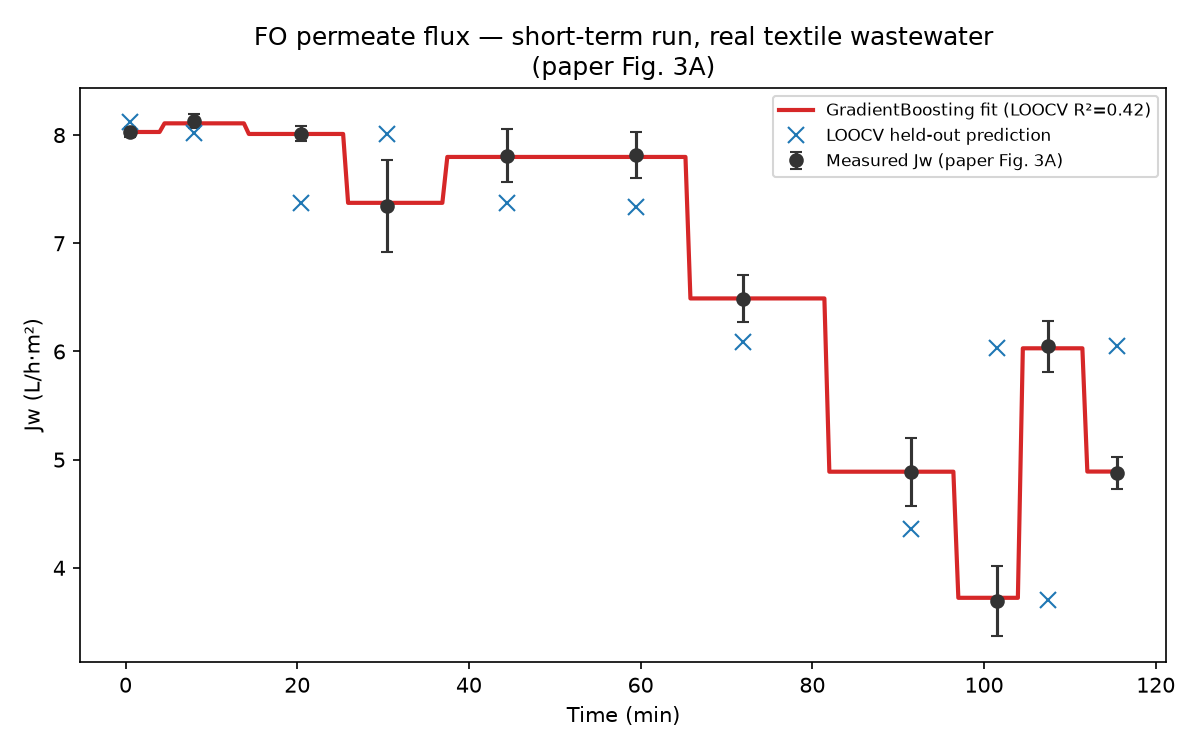
\includegraphics[width=0.92\linewidth]{plots/model1b_fo_flux_shortterm.png}
\caption{Short-term FO permeate flux during concentration of textile wastewater, corresponding to the base paper's Fig. 3A.}
\label{fig:shortterm_base}
\end{figure}

\begin{figure}[H]
\centering
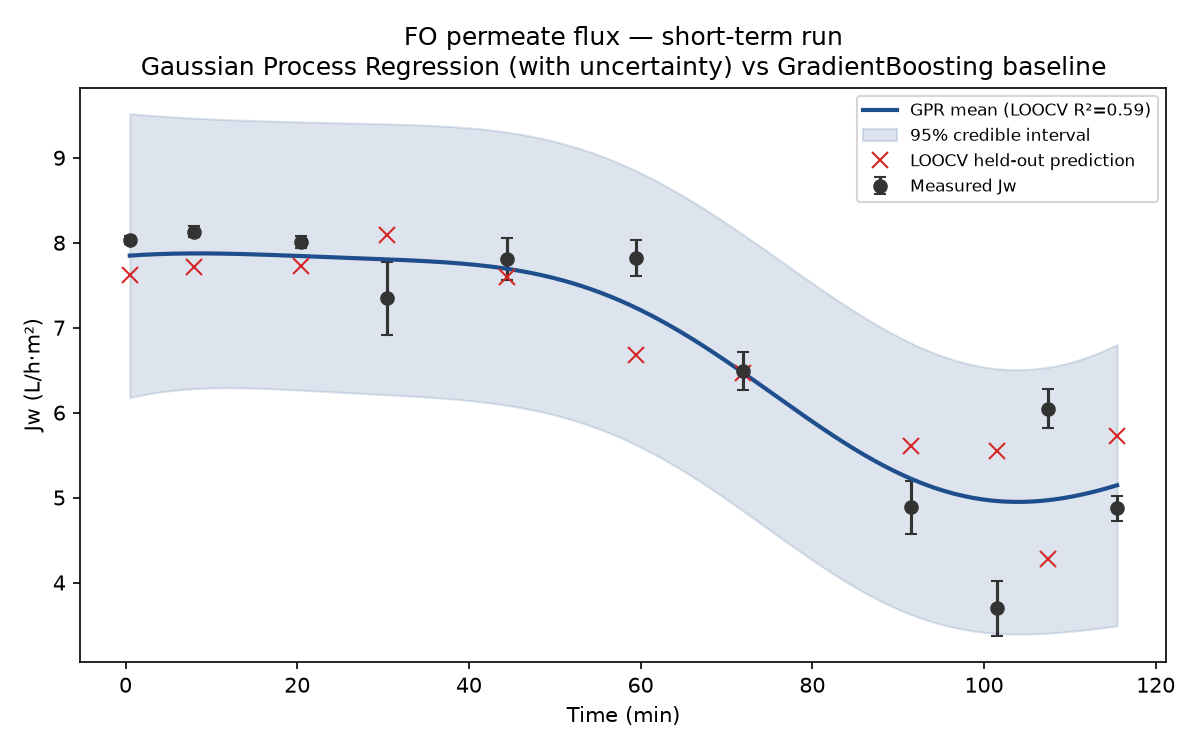
\includegraphics[width=0.92\linewidth]{plots/model1b_improved_gpr.png}
\caption{Gaussian Process Regression for short-term FO flux with 95\% credible interval and LOOCV held-out predictions.}
\label{fig:shortterm_gpr}
\end{figure}

\subsection{RO Rejection and Physical Extrapolation}
The baseline polynomial and the solution-diffusion model both describe the three calibration points reasonably well. However, with only three points, calibration fit is not the decisive test. The relevant question is whether the model remains physically meaningful outside the 30--50 bar range. The fitted solution-diffusion parameters were $A=1.0000$ and $B=0.15052$, with $R^2=0.9773$ on the calibration points. At 50 bar, the physical model predicted 99.40\% rejection, close to the base paper's 99.2\% value. At 70 bar, the physical model remained bounded at 99.67\%, while the polynomial dropped to 95.66\%. At 20 bar, below the approximate osmotic-pressure limit, the physical model correctly returned 0.00\%, while the polynomial still predicted 94.12\% rejection.

\begin{figure}[H]
\centering
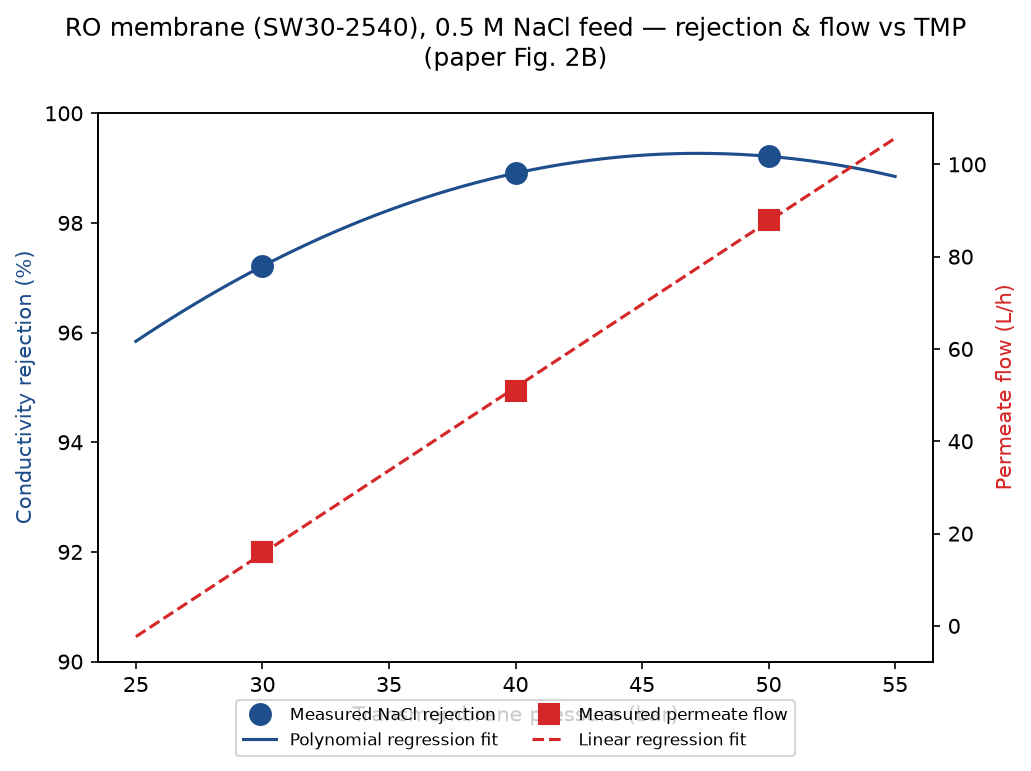
\includegraphics[width=0.82\linewidth]{plots/model2_ro_rejection.png}
\caption{RO conductivity rejection and permeate flow versus TMP for the SW30-2540 membrane, corresponding to the base paper's Fig. 2B.}
\label{fig:ro_base}
\end{figure}

\begin{figure}[H]
\centering
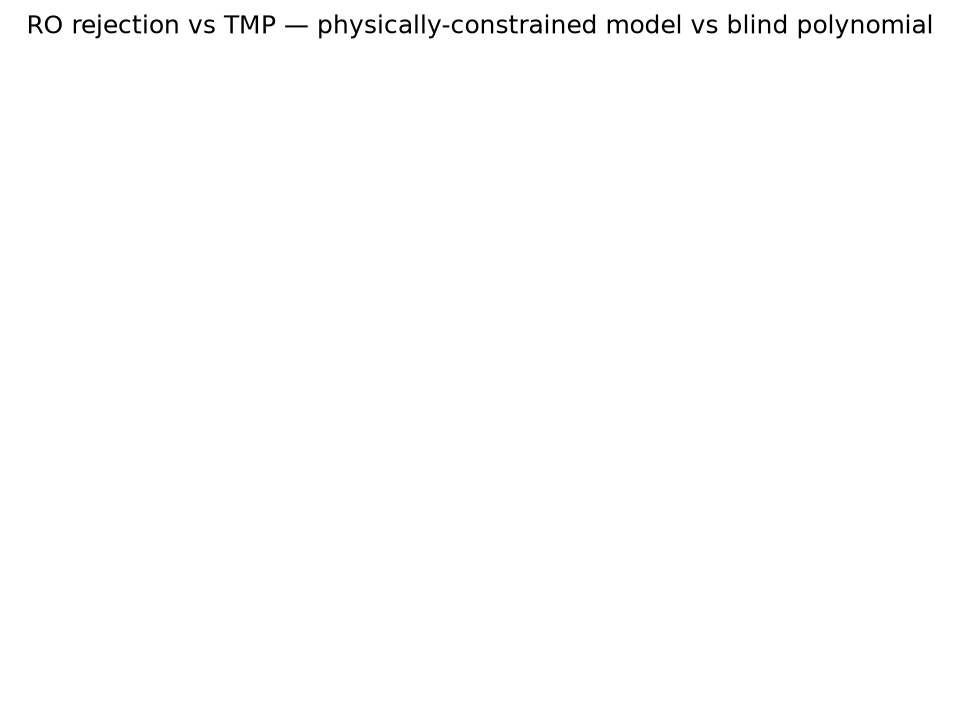
\includegraphics[width=0.92\linewidth]{plots/model2_improved_physical.png}
\caption{Physically constrained RO rejection model compared with the degree-2 polynomial baseline. The solution-diffusion model preserves sensible behavior outside the calibration range.}
\label{fig:ro_physical}
\end{figure}

\subsection{Solute Tracking Across Streams}
The base paper reported strong COD and TOC rejection and characterized feed and draw streams across recovery levels. In the project model, a single concentration-factor regression captured feed-side concentration well but failed for the draw-out stream. This failure is expected: draw-out chemistry is regulated by continuous RO regeneration and should not necessarily scale with feed concentration. Similar distinctions between feed-side concentration, draw-solution behavior, and downstream RO recovery are important across FO-RO hybrid designs \cite{b7}.

\begin{table}[H]
\centering
\caption{Comparison of original solute interpretation and modified solute-modeling results.}
\label{tab:original_modified_solute}
\begin{tabular}{p{0.18\linewidth}p{0.31\linewidth}p{0.37\linewidth}}
\toprule
Stream or target & Original research paper interpretation & Modified project interpretation \\
\midrule
Feed-in stream & Feed concentration increased with water recovery as wastewater became more concentrated. & Linear concentration-factor regression remained strongest for feed-in behavior, with LOOCV $R^2$ values of 0.979 for TOC, 0.982 for TDS, and 0.949 for conductivity. \\
Feed-out stream & Feed-out quality followed the concentrated feed behavior after contact with the FO module. & Model choice was mixed: linear-CF was better for TOC ($R^2=0.893$), while GPR was better for TDS ($R^2=0.860$) and conductivity ($R^2=0.949$). \\
Draw-out stream & Draw solution quality remained comparatively stable because RO continuously regenerated the saline draw solution. & Linear-CF assumptions failed for draw-out behavior. GPR improved draw-out TOC from $R^2=-2.071$ to $-0.534$, TDS from $-2.252$ to $-1.196$, and conductivity from $-2.259$ to $-1.219$. \\
Organic rejection & COD and TOC rejection were reported above 99\%, confirming strong retention of organic contaminants. & The modeling results support the same physical interpretation: draw-out solute behavior should not be forced to follow feed-side concentration-factor scaling. \\
\bottomrule
\end{tabular}
\end{table}

\begin{figure}[H]
\centering
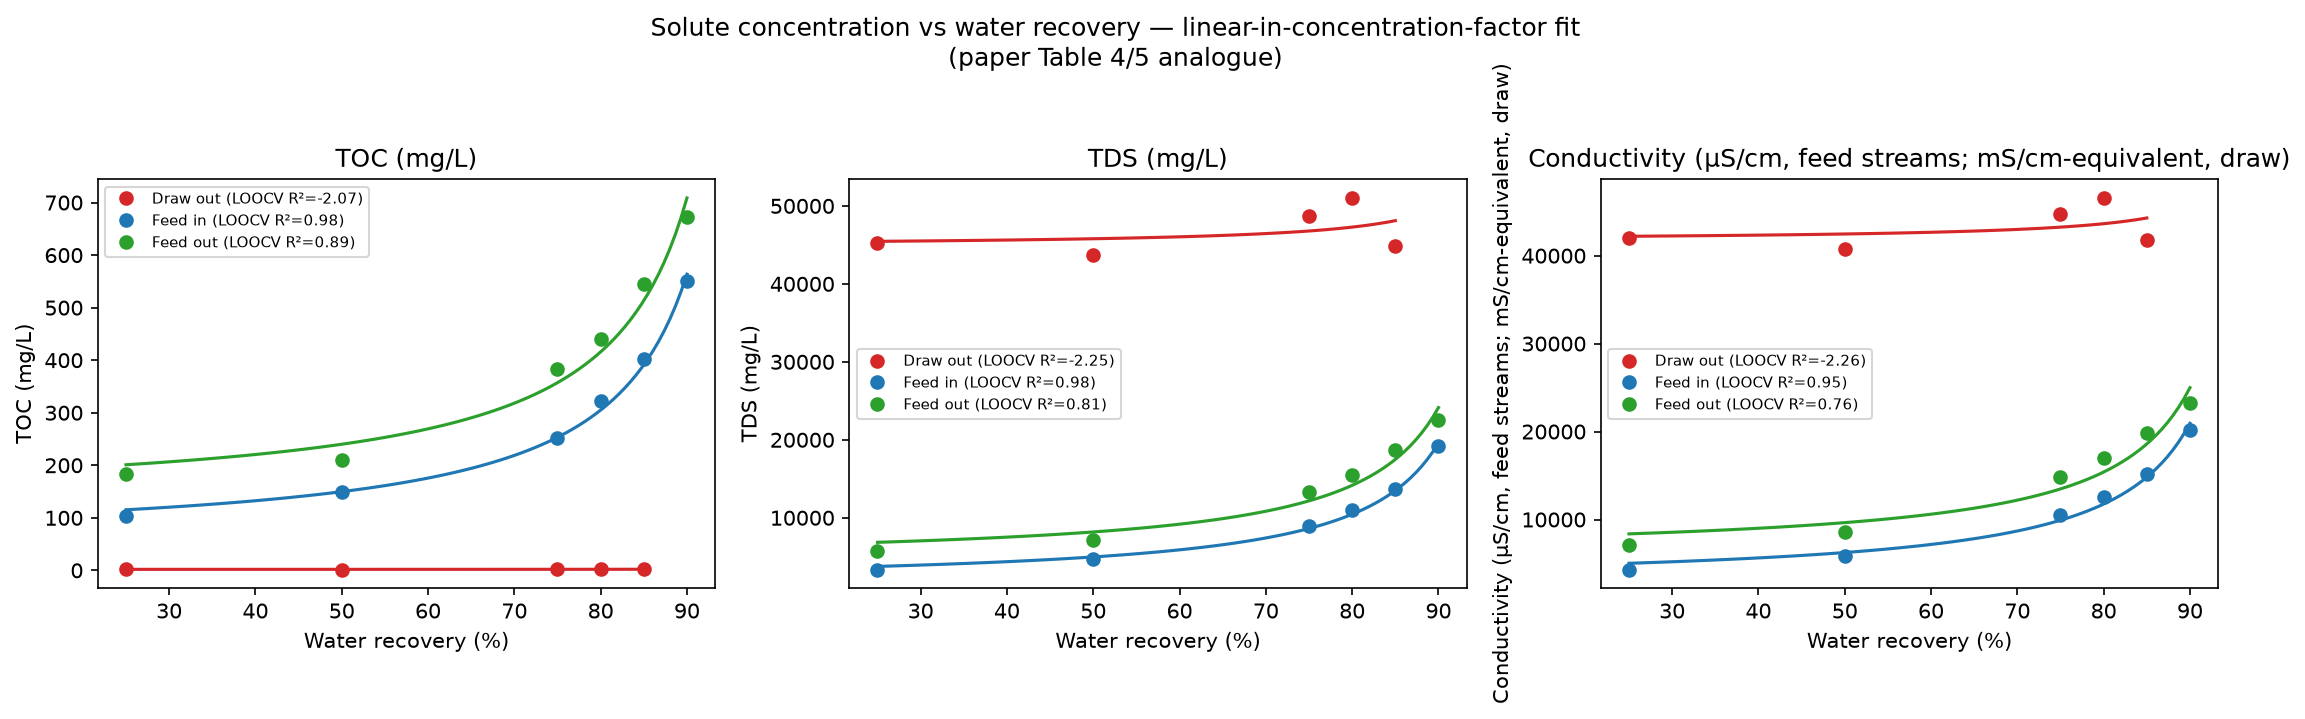
\includegraphics[width=0.98\linewidth]{plots/model3_toc_tds_cond.png}
\caption{Baseline concentration-factor model for TOC, TDS, and conductivity across water recovery levels.}
\label{fig:solute_base}
\end{figure}

\begin{figure}[H]
\centering
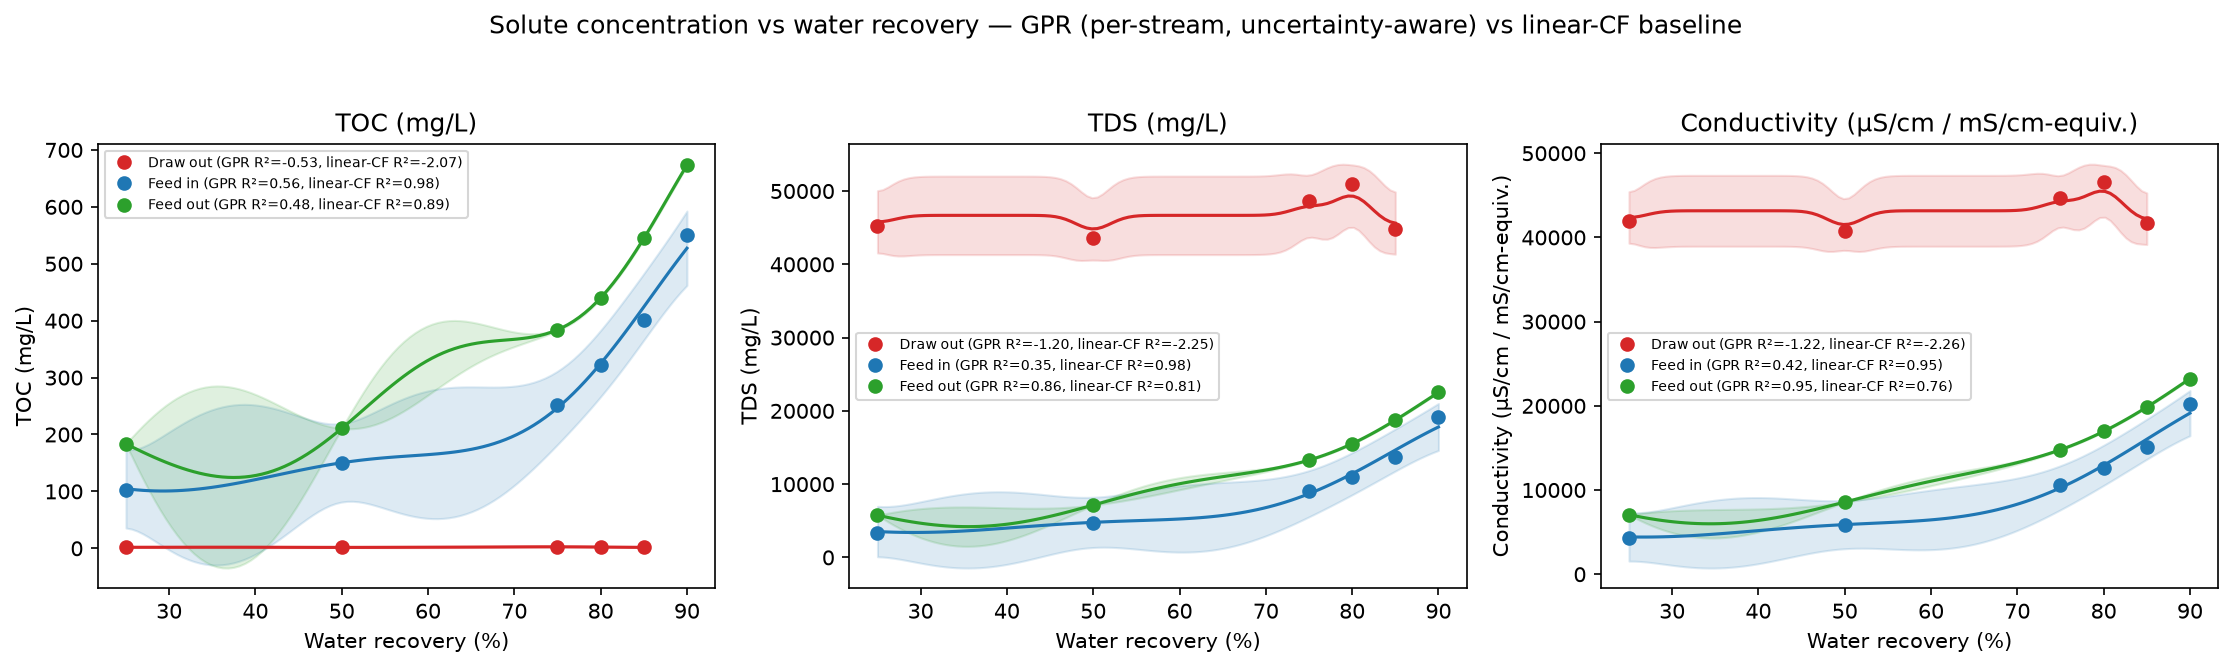
\includegraphics[width=0.98\linewidth]{plots/model3_improved_gpr.png}
\caption{Per-stream GPR model for TOC, TDS, and conductivity with uncertainty bands and comparison against the linear concentration-factor baseline.}
\label{fig:solute_gpr}
\end{figure}

\begin{table}[H]
\centering
\caption{LOOCV $R^2$ comparison for solute-tracking models.}
\label{tab:solute_models}
\begin{tabular}{llcc}
\toprule
Stream & Target & Linear CF $R^2$ & GPR $R^2$ \\
\midrule
Draw out & TOC & $-2.071$ & $-0.534$ \\
Feed in & TOC & $0.979$ & $0.560$ \\
Feed out & TOC & $0.893$ & $0.478$ \\
Draw out & TDS & $-2.252$ & $-1.196$ \\
Feed in & TDS & $0.982$ & $0.350$ \\
Feed out & TDS & $0.813$ & $0.860$ \\
Draw out & Conductivity & $-2.259$ & $-1.219$ \\
Feed in & Conductivity & $0.949$ & $0.423$ \\
Feed out & Conductivity & $0.759$ & $0.949$ \\
\bottomrule
\end{tabular}
\end{table}

The draw-out stream improved consistently under GPR, although the scores remained negative because the sample size is extremely small and the response is nearly flat relative to the feed streams. Feed-in behavior remained better described by the concentration-factor model, while feed-out behavior was mixed. This confirms that model selection should be stream-specific rather than uniform across the whole FO-RO system.

\section{Conclusion}
This project used the coupled FO-RO textile-wastewater study as a base experimental system and developed a process-aware machine-learning reinterpretation of its data. The main correction was methodological: each model was selected according to the structure and physical constraints of its dataset. Time-series validation and engineered temporal features improved long-term FO flux prediction; GPR improved sparse short-term flux interpolation and provided uncertainty bands; a solution-diffusion model prevented unphysical RO rejection extrapolation; and per-stream solute modeling showed that feed and draw streams require different assumptions. Overall, the results show that the best modeling workflow for membrane processes is not the most flexible algorithm in isolation, but the model whose validation strategy and inductive bias match the underlying transport process.

\section*{Code Availability}
The project notebooks, scripts, processed datasets, model outputs, and generated figures are available in the GitHub repository: \url{https://github.com/DaDicaso/FML_ResearchPaper}.

\section*{Use of AI Tools}
AI-assisted tools, including ChatGPT, Gemini, and Claude, were used to support literature organization, manuscript drafting, language refinement, coding assistance, and figure/table preparation. The authors reviewed, verified, and remain responsible for the final content, calculations, interpretations, and conclusions presented in this paper.

\section*{Declaration of Competing Interest}
The authors declare no competing financial interests.

\begin{thebibliography}{00}
\bibitem{b1} C. M. S\'anchez-Ar\'evalo, L. Garc\'ia-Suarez, M. S. Camilleri-Rumbau, J. Vogel, S. \'Alvarez-Blanco, M. C. Vincent-Vela, and B. Cuartas-Uribe, ``Continuous regeneration of the draw solution in textile wastewater treatment using a combination of simultaneous forward osmosis and reverse osmosis,'' \textit{Chemical Engineering and Processing - Process Intensification}, vol. 221, p. 110689, 2026, doi: 10.1016/j.cep.2025.110689.
\bibitem{b2} D. A. Yaseen and M. Scholz, ``Textile dye wastewater characteristics and constituents of synthetic effluents: a critical review,'' \textit{International Journal of Environmental Science and Technology}, vol. 16, pp. 1193--1226, 2019, doi: 10.1007/s13762-018-2130-z.
\bibitem{b3} N. Jahan, M. Tahmid, A. Z. Shoronika, A. Fariha, H. Roy, M. N. Pervez, Y. Cai, V. Naddeo, and M. S. Islam, ``A comprehensive review on the sustainable treatment of textile wastewater: zero liquid discharge and resource recovery perspectives,'' \textit{Sustainability}, vol. 14, p. 15398, 2022, doi: 10.3390/su142215398.
\bibitem{b4} Z. Zeitoun and N. Y. Selem, ``A comprehensive review on textile wastewater treatment by coupling TiO$_2$ with PVDF membrane,'' \textit{Bulletin of the National Research Centre}, vol. 47, article 153, 2023, doi: 10.1186/s42269-023-01131-9.
\bibitem{b5} C. Pinto, A. Fernandes, A. Lopes, M. J. Nunes, A. Ba\'ia, L. Cir\'iaco, and M. J. Pacheco, ``Reuse of textile dyeing wastewater treated by electrooxidation,'' \textit{Water}, vol. 14, p. 1084, 2022, doi: 10.3390/w14071084.
\bibitem{b6} C. Wei, Y. Lao, R. Ouyang, G. Zhang, G. Huang, F. Deng, Q. Tan, G. Lin, and H. Zhou, ``Evaluation of different reverse osmosis membranes for textile dyeing and finishing wastewater reuse,'' \textit{Membranes}, vol. 13, p. 420, 2023, doi: 10.3390/membranes13040420.
\bibitem{b7} S.-J. Im, S. Jeong, and A. Jang, ``Forward osmosis (FO)-reverse osmosis (RO) hybrid process incorporated with hollow fiber FO,'' \textit{npj Clean Water}, vol. 4, article 51, 2021, doi: 10.1038/s41545-021-00143-0.
\bibitem{b8} L. Wojn\'arovits, R. Homlok, K. Kov\'acs, A. Tegze, and E. Tak\'acs, ``Wastewater characterization: chemical oxygen demand or total organic carbon content measurement?'' \textit{Molecules}, vol. 29, p. 405, 2024, doi: 10.3390/molecules29020405.
\bibitem{b9} J. A. Aguilar-Torrej\'on, P. Balderas-Hern\'andez, G. Roa-Morales, C. E. Barrera-D\'iaz, I. Rodr\'iguez-Torres, and T. Torres-Blancas, ``Relationship, importance, and development of analytical techniques: COD, BOD, and TOC in water--an overview through time,'' \textit{SN Applied Sciences}, vol. 5, p. 118, 2023, doi: 10.1007/s42452-023-05318-7.
\bibitem{b10} X. Wu, C. H. Lau, B. K. Pramanik, J. Zhang, and Z. Xie, ``State-of-the-art and opportunities for forward osmosis in sewage concentration and wastewater treatment,'' \textit{Membranes}, vol. 11, p. 305, 2021, doi: 10.3390/membranes11050305.
\bibitem{b11} Y. Xu, Y. Zhu, Z. Chen, J. Zhu, and G. Chen, ``A comprehensive review on forward osmosis water treatment: recent advances and prospects of membranes and draw solutes,'' \textit{International Journal of Environmental Research and Public Health}, vol. 19, p. 8215, 2022, doi: 10.3390/ijerph19138215.
\bibitem{b12} P. S. Goh, A. F. Ismail, B. C. Ng, and M. S. Abdullah, ``Recent progresses of forward osmosis membranes formulation and design for wastewater treatment,'' \textit{Water}, vol. 11, p. 2043, 2019, doi: 10.3390/w11102043.
\bibitem{b13} L. Li, W. Shi, and S. Yu, ``Research on forward osmosis membrane technology still needs improvement in water recovery and wastewater treatment,'' \textit{Water}, vol. 12, p. 107, 2020, doi: 10.3390/w12010107.
\bibitem{b14} M. Mohammadifakhr, J. de Grooth, H. D. W. Roesink, and A. J. B. Kemperman, ``Forward osmosis: a critical review,'' \textit{Processes}, vol. 8, p. 404, 2020, doi: 10.3390/pr8040404.
\bibitem{b15} Z. Frontistis, G. Lykogiannis, and A. Sarmpanis, ``Machine learning implementation in membrane bioreactor systems: progress, challenges, and future perspectives: a review,'' \textit{Environments}, vol. 10, p. 127, 2023, doi: 10.3390/environments10070127.
\end{thebibliography}

\end{document}
